\chapter{Model Driven Engineering}
\label{chapter:mde}

% generatoren -> bessere softwareentwicklung
Model Driven Engineering (MDE) and OMG's Model Driven Architecture (MDA) \cite{mdaguide} are intended to improve and accelerate software development. The motivation is that software development should focus on a program's specification instead of the implementation. By extensive use of generators the code is correct, quickly produced, reusable, conforming to standards and of high quality.

In Model Driven Engineering a number of models are used for different views on the system, each with a different level of abstraction.

\begin{enumerate}
	\item The \emph{Code} can be seen as the lowest level of abstraction.
	\item A \emph{Platform Specific Model} (PSM) is abstracting from the program code while preserving its basic concepts, like classes and methods. A popular example for this kind of model is UML Class Diagrams.
	\item The \emph{Platform Independent Model} (PIM) is giving a very abstract view on the system. Examples for platform independent models are for instance some UML diagrams, like UML Usecases and Activity Diagrams and BPMN.
\end{enumerate}

% einfacher zu validieren, ohne sprachspezifischen overhead wie fehlerbehandlung
In Model Driven Engineering the platform independent model (PIM) is used for modeling the program's functionality from a high level view (``programming in the large''). This model is especially useful to involve stakeholders and domain experts in the development. The PIM then can be used to generate platform specific models (PSM) for further refinement and completion, while non-functional, implementation specific details, such as exception handling and resource management, do not have to be taken into account. Finally the program code is generated from the PSM. In the ideal case no manipulation of the code is necessary; it can be fully generated from the higher level models. Some tools also provide \emph{round tripping}, meaning that changes made to the code are automatically transferred to the models, keeping them up to date.

% formale modelle -> code, unterstützt inkrementelle entwicklung
When the project has to be modified, in MDE it is best practice to change the models and to regenerate the code. This way MDE encourages \emph{incremental and iterative design} and the model is kept up to date, as shown in figure \ref{fig:lifecycle}. Further the model is \emph{independent of platform and programming language}. The same model can be used to generate an equivalent program in a different language, making programs developed using MDE highly portable: When a company has to change to a different programming language or framework the new software can be generated from the same models.

\begin{figure}[htp]
	\centering
	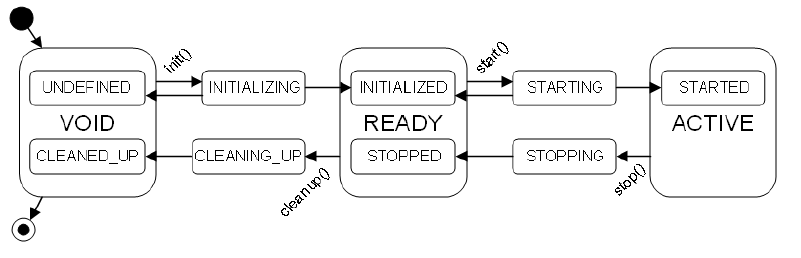
\includegraphics[width=.5\textwidth]{figures/mda/lifecycle.png}
	\caption[Model driven software development lifecycle]{Modeling and regenerating in a model driven software development lifecycle}
	\label{fig:lifecycle}
\end{figure}

% am effizientesten bei großen projekten
MDE might look like an unnecessary additional effort. Creating the different models is time-consuming and understanding the generated code and the interaction of the several generated modules can be much more difficult than understanding code written by oneself. But in projects with many developers MDE can help to provide a consistent coding style and program structure that can be understood by everyone involved in the project.

The editor developed in this thesis is about Model Driven Engineering in two ways:

\begin{enumerate}
	\item The editor has been designed and implemented using MDE.
	\item The editor can be used for developing programs using MDE.
\end{enumerate}

The following sections will describe how Model Driven Engineering can be used for the quick creation of domain specific editors using the Eclipse framework. Further existing approaches on the generation of executable programs with BPMN diagrams will be introduced as well as known problems that arise when transforming unstructured workflows to block structured programs.



\section{Using MDE for Designing Eclipse Editors}
\label{sec:mda_eclipse}

Not only can Model Driven Engineering be used for creating programs that were fully specified in a model. Another popular field of application for MDE is the generation of domain specific editors. In this case the modeling tool can be specialized on the creation of editors and thus provide a variety of modules and tools that can easily be combined to the model for a feature-rich editor for a given domain. In the Eclipse Modeling project (EMP) \cite{EMP} there are several plugins supporting the model driven development of other Eclipse editor plugins by providing both tooling and runtime support for them.

Of course one advantage of model driven architecture, the independence of a programming language, does not apply in this case, since all the programs developed this way will always be Java programs and depending on the Eclipse framework. However, Java runtime environments and the Eclipse IDE are available for every platform. And of course the result basically has to be an editor for some domain. But the domain and most of the editor's functionality can be specified with a set of models.

The frameworks introduced in this section also can create a \emph{Rich Client Platform (RCP) Application} which can be used without having Eclipse installed and running. For this purpose Eclipse can spawn a minimum copy of itself, holding only those plugins that are required for launching the editor. Such a RCP application can have a more individual look than a plugin and the platform is much smaller in size. However, this way the editor will not be capable of editing anything else than this editor's domain. The best practice might be to deploy the editor both as a plugin and a RCP, so those already having an Eclipse platform in use can use the plugin while others can use the RCP application.


\subsection{The Eclipse Modeling Framework}

The Eclipse Modeling Framework (EMF) \cite{EMF} is an implementation of \emph{Essential MOF} (EMOF). An EMF model (``Ecore'') can be generated from a UML class diagram, annotated Java interfaces or XML and in return can generate all these. From this model not only the implementations for the specified model elements can be generated, but also a full editor (see figure \ref{fig:emf1}). A good introduction to EMF can be found in \cite{emfbook}.

\begin{figure}[htp]
	\centering
	\includegraphics[width=.75\textwidth]{figures/mda/emf1.png}
	\caption[Code generation with EMF]{Creating an EMF model from other models and generating code}
	\label{fig:emf1}
\end{figure}


\subsubsection*{EMF Generated Models}

The generated implementations provide many features.

\begin{itemize}
	\item automated serialization
	\item implementation of the \emph{Observer} pattern
	\item undoable editing
	\item multiple inheritance
	\item merging of generated and handwritten code
	\item generic access to classes and attributes
	\item dynamic creation of new classes at runtime
\end{itemize}

By default the model instances can be saved persistently to XML. If the Ecore has been generated from an XSD file the serialized form will have exactly the syntax specified in the XSD. However it is also possible to provide another serialization that can be integrated in the framework as well.

Extending the class \verb|EObject| the model instances will notify their \verb|Adapters| whenever they undergo changes, e.g. when an attribute is assigned a new value. This not only enables refreshing diagrams as needed; additionally every change to an EObject can be recorded, providing undoable editing.

Since for each class in the model there is an interface and an implementation EMF models provide multiple inheritance: Several interfaces are implemented and the generator is taking care for the code duplication necessary since Java itself does not support multiple inheritance.

The generated code can be altered and extended with handwritten fields and methods. Using annotations the generator recognizes which parts shall be regenerated and what has to remain untouched.

Apart from the actual interfaces and implementation for all the classes defined in the model there will also be a single \verb|Package| class with a constant internal instance for each of the classes, attributes and references in the model (see figure \ref{fig:emf2}).

\begin{figure}[htp]
	\centering
	\includegraphics[width=.5\textwidth]{figures/mda/emf2.png}
	\caption[Ecore metamodel]{The Ecore model's internal representation (simplified subset)}
	\label{fig:emf2}
\end{figure}

Using these ``meta classes'' EMF is providing reflective access to all the classes and attributes (introspection). Thus instead of \verb|somePerson.setName("Peter")| the reflective version \verb|somePerson.eSet(FooPackage.PERSON__NAME,"Peter")| can be used. While not needed in general this can be useful for dynamically creating new classes at runtime:

\footnotesize
\begin{verbatim}
EAttribute name= EcoreFactory.eINSTANCE.createEAttribute();
name.setName("name");
name.setEType(EcorePackage.eINSTANCE.getEString());

EClass person= EcoreFactory.eINSTANCE.createEClass();
person.setName("Person");
person.getEStructuralFeatures().add(name);

EPackage myPackage= EcoreFactory.eINSTANCE.createEPackage();
myPackage.getEClassifiers().add(person);

EFactory myFactory = myPackage.getEFactoryInstance();
EObject somePerson= myFactory.create(person);
somePerson.eSet(name, "Peter");
\end{verbatim}
\normalsize

\subsubsection*{EMF Generated Editors}

%one click -> editor
Apart from a feature rich and efficient implementation of the domain model the EMF framework also can be used for generating a complete editor for it. This can be done with literally one click. The generated editor provides a semi-visual tree view for the model, undoable editing, serialization and deserialization. Like the model files the editor can be customized if necessary, too.

%RCP application
As said before an RCP application can be created, too. With the EMF generator and EMF plugin development assistants this is a matter of minutes. The resulting RCP application's size is only about 10\% of the original Eclipse application's size.


\subsection{The Graphical Modeling Framework}
\label{sec:mda_gmf}

% erzeugung von graphischen editoren basierend auf den modellen von emf
The Graphical Modeling Framework (GMF) \cite{GMF} is a promising approach to provide a framework for generating standardized feature-rich visual editors for EMF models.

A brief introduction to the GMF runtime can be found in \cite{gmf_intro,gmf_arch}. The first version, GMF 1.0, was released with the \emph{Callisto Simultaneous Release} in June 2006 and version 2.0 will be part of the \emph{Europa Simultaneous Release} scheduled for June 2007.

% verbindung von emf und gef
The Graphical Modeling Framework consists of two parts: The GMF tooling and the GMF runtime. The tooling part is providing a modeling framework for designing new editors and the runtime part eases the integration of EMF and GEF, the Graphical Editing Framework \cite{GEF} used for the editor. Additionally it receives contributions from the Eclipse Modeling Framework Technology (EMFT) project and uses \emph{EMF OCL}, \emph{EMF Validation}, \emph{EMF Query} and \emph{EMF Transaction}.

\subsubsection*{Tooling}
% gmf tooling
The tooling part is providing a set of wizards and editors for modeling the editor (see figure \ref{fig:gmftooling}) that will then be generated and use the runtime part.

\begin{figure}[htp]
	\centering
	\includegraphics[width=.75\textwidth]{figures/mda/gmftooling.png}
	\caption[The GMF Dashboard]{The \emph{GMF Dashboard} showing the various models of the GMF tooling process}
	\label{fig:gmftooling}
\end{figure}

The models and editors used for designing the GMF editor are in fact created with EMF. These are the models: \emph{Graphical Definition Model}, \emph{Tooling Definition Model}, \emph{Mapping Model} and \emph{Generator Model}. One more model, the \emph{Notation Model}, is used in the GMF runtime part.

For modeling a graphical GMF editor one starts with the editor's domain as an EMF model. Next the visual representation is defined: A figure gallery with ovals, rectangles, lines and decorators, which then are associated to nodes and connections. The third part in the GMF tooling is defining the tools to be used. Basically this will be a palette with entries for each node and connection, but also  additional menus can be defined. In the last part the domain model, the notational model and the tooling model have to be glued together in the mapping model. Additional constraints for validation can be defined here, too. Finally the generator model is created from the mapping model. It is possible to define details like file extensions, names, layouts or whether to create a plugin or a RCP application. Normally this does not require any modification by the user and the default settings can be used as well. Now the visual editor can be generated and run.

By storing the various aspects of the editor -- the graphical definition, the tooling definition and the mapping -- in separate models each part can be reused without the others. For instance it would be possible to provide different GMF editors for different views on a single domain. Each editor would use the same underlying Ecore model, graphical definition model and tooling model, but different mapping models. Further the figures designed in the graphical definition model can be exported to a separate figures plugin and reused with any GEF based editor.

\subsubsection*{Runtime features}
Aside from facilitating the integration of EMF and GEF the GMF runtime is providing many value-rich features that otherwise would have to be implemented every time anew, such as:

\begin{itemize}
	\item a node's compartments can be collapsible, so the user can hide details
	\item direct editing support for all labels in the diagram
	\item modeling assistants: popup-bars and connection handles which provide fast access to all the model elements that can be used in the current context
	\item common tools, menus, toolbars and properties, like sticky notes, zooming, coloring, arranging, auto size, printing, clipboard support, graphics export and many more
\end{itemize}

Aside from the easy generation with the GMF tooling and the many features that are provided by the GMF runtime there are also more general benefits in using GMF.

% einheitlicher look and feel, guter stil (wenn auch gewöhnungsbedürftig)
An application created with GMF automatically has a look and feel familiar to every user of the Eclipse framework. And not only the user but also the developer will profit from the unified structure of the generated editor. When first generating a GMF editor one might be discouraged by the somewhat bulky code. This is just natural and not different from when someone starts maintaining code originally written by someone else. However, since the code of each editor generated with GMF has the same structure, once familiar with GMF maintaining a GMF project will be easy, even if it was originally designed by someone else.

% zwei dateien, modell und layout
In the default configuration the editor will save diagrams in two files: One file for the model, the other for the layout information. This is where the last model mentioned earlier, the notation model, is applied. This model is holding all the layout information, like positions, colors and fonts. This way the model does not have to be enriched with layout information, like a point for a node's location or a list of points for a connection's bendpoints\footnote{while this might still be applicable for simple layouts where each node has a position and each connection some bend points, it is not for providing e.g. persistent colors and fonts}. This way the pure model file can be interpreted by other programs, too, especially when generated from a XSD. Further a new layout file can be initialized from the plain model file.

On the downside each model element has to be synchronized with it's View element when being created, moved or deleted. In GEF the only thing needed to insert a new child node is to create the node's model, set it's coordinates, insert it into its parent and make a call to \verb|refreshChildren|. In GMF the same task is more complicated.

% man profitiert von zufünftigen entwicklungen
Last not least an editor created with GMF will be maintained and enhanced even when actually no one is maintaining it: The GMF community is continuously improving the GMF framework, adding new features and fixing bugs. When a new version of GMF is available the editor can be regenerated with that new version and it will provide all the new version's features and bugfixes.

% generator + customizable
Like in EMF the generated code can be customized in many ways. When regenerating the editor due to changes in the model the generated code will be merged with those parts written by hand.



\section{Using MDE for Modeling Processes}
\label{sec:mda_process}

In this section we will look on the second aspect of Model Driven Engineering covered in this thesis: The model based creation of arbitrary programs, especially services and business processes. First we will present the major challenges in transforming BPMN diagrams to executable process models. Thereafter we will present some existing approaches and tools.


\subsection{Unstructured Workflows}
\label{sec:mda_mapUSWF}

The major challenges in transforming a BPMN business process diagram to a program arise from the fact that, while a BPMN diagram is a unstructured directed graph, most executable languages are based on structured workflows. Thus the source model has to be altered so it can be expressed in a structured form. This is not always possible, since without the restriction to structured models the source language, BPMN, has more expressive power than the target languages.

A good definition of \emph{Structured Workflow Models} (SWMs) is given in both \cite{strucWFmodeling} and \cite{taxo_unstr_wf}. The definition says the following:

\begin{enumerate}
	\item A single activity $A$ is a SWM. $A$ will be both the initial and the final activity of the SWM.
	
	\item Two SWMs $X_1$ and $X_2$ with a control flow going from the final activity of $X_1$ to the initial activity of $X_2$ are a SWM (a sequence).
	
	\item A block starting with an and-split (or-split) $S$ and ending with an and-join (or-join) $J$ with a number of SWMs $X_1$ to $X_n$ in between, with control flow going from $S$ to the initial activities of each $X_i$ and from the final activity of each $X_i$ to $J$, is a SWM (a parallel or alternative block).
	
	\item A block starting with a or-join $J$ and ending with a or-split $S$ and two SWMs $X_1$ and $X_2$ with control flow from $J$ to the initial activity of $X_1$ and from the final activity of $X_1$ to $S$ and from $S$ to the initial activity of $X_2$ and from the final activity of $X_2$ to $J$ is a SWM (a loop).
\end{enumerate}

Please have a look at figure \ref{fig:swm} for a more descriptive picture of Structured Workflow Models.

\begin{figure}[htp]
	\centering
	\includegraphics[width=1\textwidth]{figures/mda/swm.png}
	\caption[Basic Structured Workflow Models]{Basic Structured Workflow Models: Atomic Activity, Sequence, Block, Loop. Darkened nodes stand for composite parts of the workflow that have already been identified as a SWM.}
	\label{fig:swm}
\end{figure}

% arbitrary mächstiger als structured
The fact that a structured workflow model has less expressive power than an arbitrary workflow and that not every arbitrary workflow can be mapped to a semantically equivalent structured workflow can be made clear by the following: The definition of structured workflows guarantees that structured workflows do neither deadlock nor result in multiple instances of the same activity being active at the same time (also referred to as a lack of synchronization). Arbitrary workflows like BPMN diagrams \emph{can} deadlock or result in multiple instances. Thus a structured workflow does not have the same expressive power as an arbitrary workflow.

The two kinds of structural conflicts mentioned above -- deadlocks and a lack of synchronization, resulting in multiple instances -- can occur when merging sequences with an and-join, which can result in deadlocks if not all these sequences are visited in the workflow instance, or when merging sequences with a or-join, which can be the cause for a lack of synchronization, if more than one of the sequences are visited in the workflow instance.

For the transformation of a unstructured workflow (1) structured workflows have to be recognized in the directed graph and (2) if the directed graph is not a structured workflow it has to be altered accordingly.


\subsubsection*{Validation and Identification of Structured Workflows}

% erkennung über reduktion mit an die definition angelehnten regeln
One possibility for validating whether a directed graph is a structured workflow is to create a set of rules based on the definition given earlier in this section. Firstly every atomic activity is associated by a reference object. Then rules for identifying sequences, blocks and loops are applied as long as possible in a bottom-up way, \emph{reducing} the involved activities' references (or the graph itself). If in the end only one workflow reference is left -- that is, if all the smaller structured workflows are successfully combined to one -- the diagram as a whole is a structured workflow.

In \cite{graRedIdStrConfl,analProcGraRedTech} a set of rules is introduced for identifying not only workflows that follow a block structure but also workflows that are acyclic directed graphs while not having deadlocks or a lack of synchronization. The rules are applied iteratively, reducing the workflow by simplifying those parts that are definitely correct, for instance when there is a node with exactly one incoming and outgoing control flow the node is removed and the flow spans from the node predecessor to it's successor.

If the workflow can be reduced to a trivial workflow (that is, an empty or atomic workflow) then the workflow is correct in the sense that it is free of structural conflicts. Otherwise, if the workflow can not be reduced to a trivial workflow, it must contain at least one structural conflict. The algorithm has been implemented in a tool that can import diagrams from IBM's \emph{MQ Workflow}, validate and re-export them.

In \cite{novelGraphReduction} it has been shown that the algorithm is not complete and that there are correct workflow models that can not be completely reduced by the algorithm. The algorithm has been extended and its correctness and completeness have been proved.

\subsubsection*{Transformation of Unstructured Workflows}

The transformation of unstructured workflows to structured workflows is much more complicated than identifying existing structured workflows (and transforming them to other workflow languages).

% transformation sehr kompliziert...
The reason is that there are a lot more patterns of unstructured workflows than for structured workflows. As written before all structured workflows following certain criteria can be identified with some simple rules. In \cite{strucWFmodeling} and \cite{taxo_unstr_wf} various patterns of unstructured control flow have been identified: Entry in and exit from a block (loop) structures, overlapping blocks (loops), one split (join) for multiple joins (splits), and many others. Approaches for structuring these patterns were given, too. However these solutions are quite complicated and it is not known to the author in how far these approaches have been implemented yet.

% ohne parallelism: jedes AWM in SWM überführbar, parallelism -> deadlocks und MI
Further it has been shown that while each unstructured workflow without parallelism can be translated to a structured workflow the introduction of parallelism can cause both deadlocks and multiple instances and that there are arbitrary workflows that can not be modeled in a structured way at all \cite[Theorem 2]{strucWFmodeling}. In some languages, such as BPEL, multiple instances can be achieved by spawning processes, but it is obvious that such programs will be hard to understand and to maintain. Further BPEL's \verb|link| element can be used for modeling some sorts of overlapping parallel structures.

Despite these exceptions every arbitrary workflow model has to be changed to a structured workflow model before being mapped to a structured target language. Basically this can be done by the modeler as well, but it is much more convenient to have this step automated.

% node-duplication, auxiliary variables -> unübersichtlicher, schlechter wartbar (beispiel-bild)
As stated in \cite{strucWFmodeling} the transformation of a unstructured workflow to a structured workflow can require \emph{node duplication} and the use of \emph{auxiliary variables}. In the case of node duplication an activity or a whole workflow segment has to be duplicated and placed in two concurring branches of the structured workflow that were interconnected in the unstructured workflow. When using auxiliary variables a new variable, usually of type \verb|boolean|, has to be declared. The variable is set in one branch of a concurrency structure and can later be read, remembering in which branch the workflow was earlier (and, in the unstructured version of the workflow, still would be in).

% conclusion: modellierung als AWM, dann validierung und export nach SWM
Both approaches make the workflow very hard to understand and to maintain. Thus it is advantageous not to restrict the user to create structured workflows but to allow both structured and unstructured workflows and to transform unstructured workflows to a equivalent structured workflow model later.

% bisimulation
For the validation of the resulting workflow a \emph{bisimulation} can be made, meaning that both the source and target workflows are simulated manually or programmatically. If in each situation the target workflow can simulate the source workflow\footnote{meaning that when the source workflow is in state A and has active transitions to the states B, C and D then the target workflow also has to be in state A with active transitions to exactly the states B, C and D} and vice versa then the workflows are equivalent.

% goto-elimination
In \cite{untanglingCyclicFlows} another rule-based approach for handling unstructured cyclic flows, that is, cyclic workflow structures with more than one entry and / or exit points, is presented. The approach is based on a method that has been introduced about forty years ago and was originally invented for the elimination of \verb|goto| statements in compiler theory.

By understanding control flow in workflow diagrams as just another form of \verb|goto| statements the idea could be transfered to cyclic workflows. After transforming an unstructured cyclic example workflow to a structured cyclic workflow a possible application on a BPEL workflow containing invalid cyclic links has been shown. The authors state that due to the simplicity of their algorithm the restriction to acyclic \verb|link|s in BPEL could be dropped entirely.


\subsection{From BPMN to BPEL}

The motivation of BPMN was to facilitate the creation of business processes and to put an end to the numerous proprietary process modeling notations used in various BPEL process design tools. Thus the BPMN specification already comes with a recommendation on a mapping of BPMN to BPEL \cite[Chapter 11]{spec_bpmn}. Still this mapping does not cover all aspects of BPMN and there are elements and attributes that can not be mapped to BPEL, such as Transactions and Ad-Hoc Processes.

In the mapping proposed in the BPMN specification control flow modeled with Sequence Flows is mapped to structured elements, such as BPEL Sequences, Flows and While-Loops. Note that there are other proposals for mappings, too. White, the author of the original mapping, presents an alternative mapping \cite{bpmnToModelBpel}. In this mapping all elements are contained in a single Flow element. Sequence Flows are mapped to Links, connecting the Activities. Only the While element is still needed for loops, since Links must not be cyclic in BPEL.

In \cite{trafoStdProcMod2BPEL} another extension of the original mapping from BPMN to BPEL is shown. The authors show that some otherwise problematic workflow patterns, such as arbitrary cycles and multiple instances, can be mapped to BPEL using the rarely used Event Handler element. Extensions to other patterns such as deferred choice and cancellation are planned.

% liste auf omg-website
A list of existing implementations of BPMN can be found at \url{http://www.bpmn.org/BPMN_Supporters.htm}. Note however that not necessarily all of those implementations also provide export functionality.


\subsection{From BPMN to Agents}

% aamas-papers nach agents-ref scannen, insb. konferenzen und workshops

% ziemlich neu, wenig referenzen
The transformation of BPMN or other process modeling notations to agent concepts is a relatively new field of research. To the author's best knowledge only few approaches have been made so far.

In \cite{bpmn2agents} we made the first step towards a transformation from BPMN to the JIAC framework, by giving a formal definition of a \emph{BPMN Normal Form} and a mapping from this normal form to petri nets, which then can be validated with respect to termination, relevance of places and boundedness.

% workflow composition mit daml-planner, services als daml-s beschrieben, hoher aufwand
Following a different approach, Vidal et al. \cite{vidal04a} propose to replace the static BPEL workflows used today by those dynamically composed by an AI planner and executed by agents. For this each web-service would need to have a machine-readable description of its precondition, effect, input and output, for instance based on the Web Ontology Language for Web Services (OWL-S) \cite{spec_owls}. As an example the planning of a vacation is given, including the booking of a flight and hotel, using existing web services but without requiring the user to care about all the details. Still the computational complexity is a problem, especially in the case of conditions and loops, when the plan would have to be reconsidered. Another possibility would be to describe the rough workflow using BPEL or the likes, using agents and planning to care only about the details, like which weather service to choose, e.g. based on other agents' ratings.
\\
\\

In this chapter the basic concepts of Model Driven Engineering have been introduced as well as how they can be applied for the creation of editors and the generation of executable programs from workflows. In the next chapter some transformation tools which can be used for that purpose will be introduced briefly. The EMT framework, being used in this thesis, will be described in detail.
